\subsection{Analysis}
\begin{frame}{Quicksort Recurrence}
  \begin{block}{Expected Comparisons}
    \[
      T(n) \leq n + \frac{1}{n} \sum_{i=1}^n (T(i-1) + T(n-i))
    \]

    Base case: $T(1) = 0$

    Solution: $T(n) = O(n \log n)$
  \end{block}
\end{frame}

\begin{frame}{Slick Analysis: Indicator Variables}
  \begin{itemize}
    \item $Q(A)$: Number of comparisons on input $A$

    \item $X_{ij}$: Indicator for whether elements $i$ and $j$ are compared

    \item $E[Q(A)] = \sum_{i<j} Pr[R_{ij}]$

    \item $Pr[R_{ij}] = \frac{2}{j-i+1}$
  \end{itemize}

  \begin{block}{Visualization}
    \begin{center}
      % Insert comparison probability diagram here
      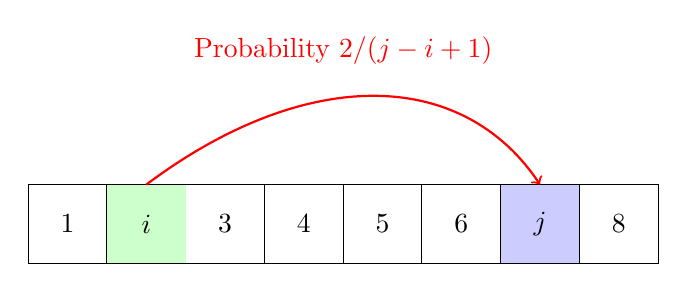
\begin{tikzpicture}[scale=1, every node/.style={scale=1}]
        % Draw array boxes
        \foreach \i in {1,...,8} {
            \draw (\i,0) rectangle (\i+1,1);
            \node at (\i+0.5,0.5) {\i};
          }
        % Highlight i and j
        \fill[green!20] (2,0) rectangle (3,1);
        \fill[blue!20] (7,0) rectangle (8,1);
        \node at (2.5,0.5) {$i$};
        \node at (7.5,0.5) {$j$};
        % Draw arc between i and j
        \draw[thick,red,->] (2.5,1) .. controls (4.5,2.5) and (6.5,2.5) .. (7.5,1);
        \node[red] at (5,2.7) {Probability $2/(j-i+1)$};
      \end{tikzpicture}
    \end{center}
  \end{block}
\end{frame}

\begin{frame}{Harmonic Numbers in Analysis}
  \begin{block}{Harmonic Number}
    $H_n = \sum_{i=1}^n \frac{1}{i} = \Theta(\log n)$
  \end{block}

  \begin{block}{Summation in Quicksort}
    $E[Q(A)] \leq 2nH_n = O(n \log n)$
  \end{block}
\end{frame}